\chapter{Конструкторская часть}

В этой части представляются требования к программе,

\section{Диаграмма прецендентов}

Диаграмма прецендентов представлена на рисунке~\ref{fig:use-case-diagram}.

\begin{figure}[h]
	\centering
	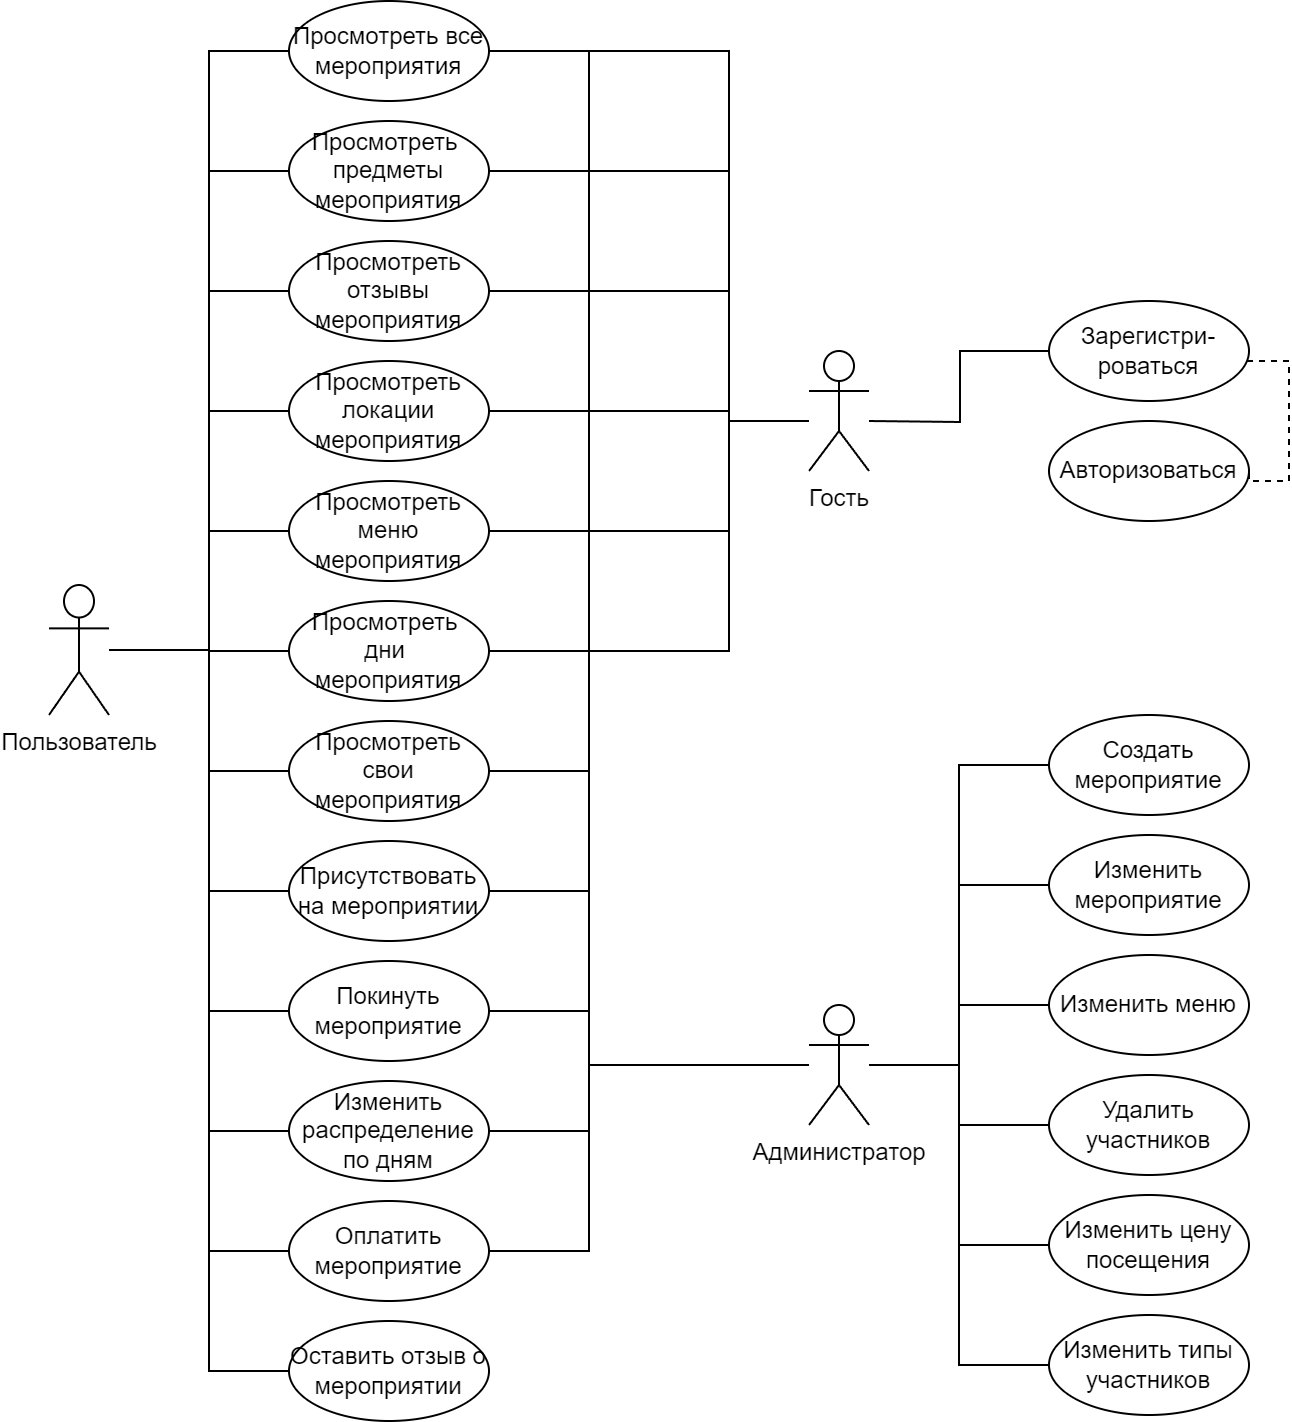
\includegraphics[width=1\textwidth]{images/use-case-diagram.png}
	\caption{Диаграмма прецендентов} 
	\label{fig:use-case-diagram} 
\end{figure}

\section{Описание сущностей базы данных}

На основе данных, представленных в таблице~\ref{tbl:data-groups}, можно определить таблицы, которые должны быть включены в базу данных:
\begin{enumerate}
	\item locations -- таблица локаций;
	\item events -- таблица мероприятий;
	\item persons -- таблица участников мероприятий;
	\item days -- таблица дней мероприятий;
	\item menu -- таблица меню дней мероприятий;
	\item items -- таблица предметов меню;
	\item feedbacks -- таблица отзывов участников;
	\item users -- таблица пользователей.
\end{enumerate}

На основе информации о выбранной СУБД и ER-диаграммы на рисунке~\ref{fig:er-diagram} будут определены структуры столбцов, их типы и ограничения для каждой таблицы, которые представлены в таблицах~\ref{tbl:locations}-\ref{tbl:users}.

\begin{table}[h]
	\centering
	\caption{Информация о таблице локаций}
	\begin{tabularx}{\textwidth}{|p{2.6cm}|X|p{6cm}|X|}
		\hline
		\textbf{Атрибут} & \textbf{Тип данных} & \textbf{Ограничения} & \textbf{Сведение} \\
		\hline
		location\_id & UUID & NOT~NULL, \newline PRIMARY~KEY & Идентификатор локации \\
		\hline
		name & VARCHAR(255) & NOT~NULL & Название \\
		\hline
		description & TEXT & NOT~NULL & Описание \\
		\hline
		price & NUMERIC & NOT~NULL, \newline CHECK~(price~>=~0) & Цена аренды на 1 день \\
		\hline
		capacity & INT & NOT~NULL, \newline CHECK~(capacity~>=~0) & Вместимость \\
		\hline
	\end{tabularx}
	\label{tbl:locations}
\end{table}

\begin{table}[h]
	\centering
	\caption{Информация о таблице мероприятий}
	\begin{tabularx}{\textwidth}{|p{2.6cm}|X|p{6cm}|X|}
		\hline
		\textbf{Атрибут} & \textbf{Тип данных} & \textbf{Ограничения} & \textbf{Сведение} \\
		\hline
		event\_id & UUID & NOT~NULL, \newline PRIMARY~KEY & Идентификатор мероприятия \\
		\hline
		name & VARCHAR(255) & NOT~NULL & Название \\
		\hline
		description & TEXT & NOT~NULL & Описание \\
		\hline
		date & DATE & NOT~NULL & Дата \\
		\hline
		person\_count & INT & NOT~NULL, \newline CHECK~(person\_count~>=~0) & Количество участников \\
		\hline
		days\_count & INT & NOT~NULL, \newline CHECK~(days\_count~>~0) & Количество дней \\
		\hline
		percent & NUMERIC & NOT~NULL, \newline CHECK~(percent~>=~0) & Наценка на посещение в процентах \\
		\hline
		rating & NUMERIC & NOT~NULL, \newline CHECK (rating~BETWEEN~0~AND~10) & Рейтинг \\
		\hline
	\end{tabularx}
	\label{tbl:events}
\end{table}

\begin{table}[h]
	\centering
	\caption{Информация о таблице дней мероприятий}
	\begin{tabularx}{\textwidth}{|p{2.6cm}|X|p{6cm}|X|}
		\hline
		\textbf{Атрибут} & \textbf{Тип данных} & \textbf{Ограничения} & \textbf{Сведение} \\
		\hline
		day\_id & UUID & NOT~NULL, \newline PRIMARY~KEY & Идентификатор дня мероприятия \\
		\hline
		name & VARCHAR(255) & NOT~NULL & Название \\
		\hline
		sequence\_ number & INT & NOT~NULL, \newline CHECK (sequence\_number~>~0) & Порядковый номер \\
		\hline
		description & TEXT & NOT~NULL & Описание \\
		\hline
		price & NUMERIC & NOT~NULL, \newline CHECK~(price~>=~0) & Цена посещения \\
		\hline
	\end{tabularx}
	\label{tbl:days}
\end{table}

\begin{table}[h]
	\centering
	\caption{Информация о таблице участников мероприятий}
	\begin{tabularx}{\textwidth}{|p{2.6cm}|X|p{6cm}|X|}
		\hline
		\textbf{Атрибут} & \textbf{Тип данных} & \textbf{Ограничения} & \textbf{Сведение} \\
		\hline
		person\_id & UUID & NOT~NULL, \newline PRIMARY~KEY & Идентификатор участника \\
		\hline
		name & VARCHAR(255) & NOT~NULL & Имя \\
		\hline
		type & ENUM & NOT~NULL & Тип \\
		\hline
		paid & BOOL & NOT~NULL & Факт оплаты \\
		\hline
	\end{tabularx}
	\label{tbl:persons}
\end{table}

\begin{table}[h]
	\centering
	\caption{Информация о таблице меню дней мероприятий}
	\begin{tabularx}{\textwidth}{|p{2.6cm}|X|p{6cm}|X|}
		\hline
		\textbf{Атрибут} & \textbf{Тип данных} & \textbf{Ограничения} & \textbf{Сведение} \\
		\hline
		menu\_id & UUID & NOT~NULL, \newline PRIMARY~KEY & Идентификатор меню \\
		\hline
		name & VARCHAR(255) & NOT~NULL & Название \\
		\hline
		cost & NUMERIC & NOT~NULL, \newline CHECK~(cost~>=~0) & Стоимость \\
		\hline
	\end{tabularx}
	\label{tbl:menu}
\end{table}

\begin{table}[h]
	\centering
	\caption{Информация о таблице предметов меню}
	\begin{tabularx}{\textwidth}{|p{2.6cm}|X|p{6cm}|X|}
		\hline
		\textbf{Атрибут} & \textbf{Тип данных} & \textbf{Ограничения} & \textbf{Сведение} \\
		\hline
		item\_id & UUID & NOT~NULL, \newline PRIMARY~KEY & Идентификатор предмета \\
		\hline
		name & VARCHAR(255) & NOT~NULL & Название \\
		\hline
		type & ENUM & NOT~NULL & Тип \\
		\hline
		price & NUMERIC & NOT~NULL, \newline CHECK~(price~>=~0) & Цена \\
		\hline
	\end{tabularx}
	\label{tbl:items}
\end{table}

\begin{table}[h]
	\centering
	\caption{Информация о таблице отзывов}
	\begin{tabularx}{\textwidth}{|p{2.6cm}|X|p{6cm}|X|}
		\hline
		\textbf{Атрибут} & \textbf{Тип данных} & \textbf{Ограничения} & \textbf{Сведение} \\
		\hline
		feedback\_id & UUID & NOT~NULL, \newline PRIMARY~KEY & Идентификатор отзыва \\
		\hline
		event\_id & UUID & NOT~NULL, \newline FOREIGN~KEY & Идентификатор мероприятия \\
		\hline
		person\_id & UUID & NOT~NULL, \newline FOREIGN~KEY & Идентификатор участника \\
		\hline
		comment & TEXT & NOT~NULL & Комментарий \\
		\hline
		rating & NUMERIC & NOT~NULL, \newline CHECK (rating~BETWEEN~0~AND~10) & Рейтинг \\
		\hline
	\end{tabularx}
	\label{tbl:feedbacks}
\end{table}

\begin{table}[h]
	\centering
	\caption{Информация о таблице пользователей}
	\begin{tabularx}{\textwidth}{|p{2.6cm}|X|p{6cm}|X|}
		\hline
		\textbf{Атрибут} & \textbf{Тип данных} & \textbf{Ограничения} & \textbf{Сведение} \\
		\hline
		user\_id & UUID & NOT~NULL, \newline PRIMARY~KEY & Идентификатор пользователя \\
		\hline
		phone & VARCHAR(255) & NOT~NULL & Телефон \\
		\hline
		gender & ENUM & NOT~NULL & Гендер \\
		\hline
		password & VARCHAR(255) & NOT~NULL & Пароль \\
		\hline
		role & ENUM & NOT~NULL & Роль \\
		\hline
	\end{tabularx}
	\label{tbl:users}
\end{table}

\section{Ролевая модель}

\section{Алгоритм расчета цены посещения}

\section{Используемые триггеры}

\section{Архитектура приложения}

\subsection{Диаграмма потока данных}

\subsection{Диаграмма компонентов}

\subsection{Диаграмма классов}


\section{Вывод}

В конструкторской части работы были представлены требования к программе, 

\clearpage
